% Generated by book/tools/notebook_to_tex.py. Do not edit by hand.

\chapter[한국어 작은 GPT 사전학습 (TinyStories-Korean CLM)]{한국어 작은 GPT 사전학습 (TinyStories-Korean Causal LM)}

\label{ch:26}

\markboth{한국어 작은 GPT 사전학습 (TinyStories-Korean CLM)}{한국어 작은 GPT 사전학습 (TinyStories-Korean CLM)}

\chaptermeta{26_ko_tiny_gpt/26_ko_tiny_gpt.ipynb}{https://colab.research.google.com/github/yoon-gu/neuqes-101/blob/master/26_ko_tiny_gpt/26_ko_tiny_gpt.ipynb}{작은 GPT2를 한국어 BBPE 토크나이저와 TinyStories-Korean으로 from-scratch next-token 사전학습}



\index{1Korean GPT@Korean GPT}

\index{1TinyStories Korean@TinyStories-Korean}

\index{1g0ster TinyStories Korean@g0ster/TinyStories-Korean}

\index{1byte level BPE@byte-level BPE}

\index{1BBPE@BBPE}

\index{1Korean tokenizer@Korean tokenizer}

\index{1CausalLM@CausalLM}

\index{1CrossEntropyLoss@CrossEntropyLoss}

\index{1next token prediction@next-token prediction}

\index{1GPT2Config@GPT2Config}

\index{1GPT2LMHeadModel@GPT2LMHeadModel}

\index{1DataCollatorForLanguageModeling@DataCollatorForLanguageModeling}

\index{1labels 100@labels=-100}

\index{1group texts@group\_texts}

\index{1KoGPT2@KoGPT2}

\index{1skt kogpt2 base v2@skt/kogpt2-base-v2}

\index{0한국어 GPT@한국어 GPT}

\index{0한국어 토크나이저@한국어 토크나이저}

\index{0한국어 BBPE@한국어 BBPE}

\index{0한국어 TinyStories@한국어 TinyStories}

\index{0직접 사전학습@직접 사전학습}

\index{0한글 토큰화@한글 토큰화}

\index{0학습 전 생성@학습 전 생성}

\index{0학습 후 생성@학습 후 생성}

\index{0한국어 생성@한국어 생성}

\index{1BpeTrainer@BpeTrainer}

\index{1ByteLevel@ByteLevel}

\index{1ByteLevelDecoder@ByteLevelDecoder}

\index{1PreTrainedTokenizerFast@PreTrainedTokenizerFast}

\index{1special tokens@special\_tokens}

\index{1endoftext token@endoftext token}

\index{1story restoration@story restoration}

\index{1streaming dataset@streaming dataset}

\index{1Korean BBPE vs GPT 2 BPE@Korean BBPE vs GPT-2 BPE}

\index{1token length comparison@token length comparison}

\index{1random baseline@random baseline}

\index{1ln vocab@ln(vocab)}

\index{1perplexity@perplexity}

\index{1VRAM trace@VRAM trace}

\index{1model generate@model.generate}

\index{1sampling hyperparameter@sampling hyperparameter}

\index{1continual pretraining preview@continual pretraining preview}

\index{0story 복원@story 복원}

\index{0줄 단위 데이터@줄 단위 데이터}

\index{0토큰 길이 비교@토큰 길이 비교}

\index{0무작위 기준선@무작위 기준선}

\index{0한국어 사전학습@한국어 사전학습}

\index{0한국어 생성 비교@한국어 생성 비교}

\index{1KoGPT2 reference@KoGPT2 reference}

\index{0한국어 continual pretraining@한국어 continual pretraining}



\section{변화 추적표}

\begin{booktable}{26장 변화 추적표 표}{tab:ch26-01}
\begin{adjustbox}{max width=\textwidth}
\begin{tabular}{@{}llllll@{}}
\toprule
Ch & 모델 & 토크나이저 & 데이터 & Output Head & Loss \\
\midrule

23 & 작은 BERT (한국어, scratch) + 분류 head & \inlinecode{klue/bert-base} (가져옴) & NSMC 이진 & \inlinecode{Linear(H,\ 2)} & \inlinecode{CrossEntropyLoss} \\
24 & 작은 GPT2 (약 3.72M, scratch) & BPE (직접 학습, 영어, vocab 2,048) & 영어 TinyStories 30K stories & \inlinecode{Linear(H,\ V)} (LM head, weight tied) & \inlinecode{CrossEntropyLoss} (next-token) \\
25 & \inlinecode{gpt2} (124M, OpenAI WebText 사전학습) & BPE (gpt2 그대로, vocab 50,257) & 영어 TinyStories (\ref{ch:24}장과 동일) & \inlinecode{Linear(H,\ V)} (LM head 그대로) & \inlinecode{CrossEntropyLoss} (next-token) - continual pretraining \\
\textbf{26 (현재)} & \textbf{작은 GPT2 (4.22M, scratch)} & \textbf{BBPE (직접 학습, 한국어, vocab 약 4,000)} & \textbf{한국어 TinyStories 30K stories} & \textbf{\inlinecode{Linear(H,\ V)} (LM head, weight tied)} & \textbf{\inlinecode{CrossEntropyLoss} (next-token)} \\
27 (다음) & KoGPT2 (\inlinecode{skt/kogpt2-base-v2}, 125M, 대규모 한국어 사전학습) & KoGPT2 BBPE (그대로) & 한국어 TinyStories (\ref{ch:26}장과 동일) & \inlinecode{Linear(H,\ V)} (LM head 그대로) & \inlinecode{CrossEntropyLoss} (next-token) - continual pretraining \\
\bottomrule
\end{tabular}
\end{adjustbox}
\end{booktable}

전체 장 표는 \href{https://github.com/yoon-gu/neuqes-101\#챕터별-변화추적표}{루트 README} 를 참고하세요.

\begin{center}\rule{0.5\linewidth}{0.5pt}\end{center}

\section{\texorpdfstring{Phase 4 의 영어·한국어 대칭 --- \ref{ch:24}장 \(\leftrightarrow\) \ref{ch:26}장}{Phase 4 의 영어·한국어 대칭 --- 24장과 26장}}

Phase 4 는 영어 (\ref{ch:24}--\ref{ch:25}장) 와 한국어 (26-27장) 가 \emph{같은 학습 단계} 를 \emph{언어만 바꿔} 반복하는 구조입니다. \ref{ch:20}장(영어 BERT)\(\to\)\ref{ch:22}장(한국어 BERT) 의 \emph{언어 축 변화} 가 GPT 에서 그대로 반복됩니다.

\begin{booktable}{26장 Phase 4 의 영어·한국어 대칭 - 24장과 26장}{tab:ch26-02}
\begin{adjustbox}{max width=\textwidth}
\begin{tabular}{@{}lll@{}}
\toprule
학습 단계 & 영어 & \textbf{한국어} \\
\midrule

\textbf{단계 1: Pretraining} (random init \(\to\) scratch 사전학습) & \ref{ch:24}장 (작은 GPT, 영어 TinyStories) & \textbf{\ref{ch:26}장 (현재, 작은 GPT, 한국어 TinyStories)} \\
\textbf{단계 2: Continual pretraining} (사전학습 본체 + 새 데이터) & \ref{ch:25}장 (\inlinecode{gpt2} 124M + 영어 TinyStories) & 27장 (KoGPT2 125M + 한국어 TinyStories) \\
\bottomrule
\end{tabular}
\end{adjustbox}
\end{booktable}

\begin{quote}
\textbf{본 장 = 한국어 단계 1}. \ref{ch:24}장과 \emph{본체·loss·trainer·hyperparams 모두 동일}, \emph{토크나이저 학습 코퍼스 + 데이터만 한국어}. 검증 가설: \emph{언어가 달라도 작은 GPT + 30K stories from-scratch 의 학습 동역학은 비슷하다} --- \ref{ch:20}장\(\leftrightarrow\)\ref{ch:22}장 (BERT) 에서 확인한 결을 GPT 에서 재확인.
\end{quote}



\section{변경점: \ref{ch:24}장 대비}

\begin{booktable}{26장 변경점 요약}{tab:ch26-03}
\begin{adjustbox}{max width=\textwidth}
\begin{tabular}{@{}lll@{}}
\toprule
축 & \ref{ch:24}장 (영어 GPT scratch) & \ref{ch:26}장 (한국어 GPT scratch) \\
\midrule

\textbf{언어} & 영어 & \textbf{한국어} --- \emph{유일한 변화} \\
토크나이저 학습 코퍼스 & 영어 TinyStories & \textbf{한국어 TinyStories} \\
토크나이저 알고리즘 & byte-level BPE (vocab 2,048) & \textbf{byte-level BPE (BBPE, vocab 약 4,000)} - 한글은 byte 단위라 어휘를 약간 키움 \\
데이터 & \inlinecode{roneneldan/TinyStories} (영어 동화) & \textbf{\inlinecode{g0ster/TinyStories-Korean}} (한국어 번역 동화) \\
본체 구조 & \inlinecode{GPT2Config(n\_layer=4,\ n\_head=4,\ n\_embd=256)} 약 3.72M & 같은 구조, vocab 4,000으로 \textbf{4.22M} \\
모델 클래스 & \inlinecode{GPT2LMHeadModel(config)} random init & (그대로) \\
Collator & \inlinecode{DataCollatorForLanguageModeling(mlm=False)} & (그대로) \\
Loss & \inlinecode{CrossEntropyLoss} (next-token, vocab 2,048 logits) & \textbf{\inlinecode{CrossEntropyLoss}} (next-token, vocab 약 4,000 logits) \\
학습률 & 5e-4 (scratch) & (그대로) \\
산출물 & 영어 동화 풍 generation & \textbf{한국어 동화 풍 generation} \\
\bottomrule
\end{tabular}
\end{adjustbox}
\end{booktable}

\begin{quote}
\textbf{변경점 한 가지 원칙} --- Phase 4 안에서 \emph{언어 축} 만 변합니다. 본체 구조도 학습 셋업도 \ref{ch:24}장과 동일. \emph{같은 코드를 한국어 토크나이저 + 한국어 데이터로 돌렸을 때 같은 결 (말이 되는 한국어 동화) 이 나오는가} 가 본 장의 검증 포인트.
\end{quote}

\subsection{\texorpdfstring{왜 한국어는 토크나이저를 \emph{직접} 학습하나 --- \ref{ch:25}장의 결론 잇기}{왜 한국어는 토크나이저를 직접 학습하나 --- \ref{ch:25}장의 결론 잇기}}

\ref{ch:25}장에서 \inlinecode{gpt2} (영어 WebText) 의 BPE 를 \emph{그대로} 가져와 continual pretraining 했습니다. 영어는 그게 자연스럽습니다. gpt2 BPE 가 영어 어휘를 잘 커버하기 때문입니다. 하지만 \emph{영어 gpt2 BPE 로 한국어를 토큰화하면 한글이 byte 단위로 잘게 쪼개져 토큰 수가 폭증} 합니다. 이는 \ref{ch:19}장과 \ref{ch:25}장에서 확인한 cross-language 결론입니다. 그래서 한국어는 \emph{한국어 코퍼스 위에 새 토크나이저를 학습} 하는 것이 정공법입니다. 이것이 \ref{ch:26}장이 다시 \emph{scratch} 인 이유입니다. \emph{토크나이저는 본체와 운명공동체} 원칙이 한국어에서 직접 학습을 강제합니다.



\section{Phase 4 학습 4단계 표 --- \ref{ch:26}장 = 단계 1 (한국어 pretraining)}

\ref{ch:24}장에서 도입한 \emph{GPT 시대 학습 4단계} 표. 본 장은 단계 1 (pretraining) 의 \emph{한국어판} 입니다.

\begin{booktable}{26장 Phase 4 학습 4단계 표 - 26장 = 단계 1 (한국어 pretraining) 표}{tab:ch26-04}
\begin{adjustbox}{max width=\textwidth}
\begin{tabular}{@{}llllll@{}}
\toprule
단계 & 정확 용어 & 의미 & 학습 신호 (\inlinecode{labels}) & 영어 & 한국어 \\
\midrule

1 & \textbf{Pretraining} (사전학습) & random init 본체부터 일반 코퍼스로 학습 & 거의 모든 토큰 (pad 만 \inlinecode{-100}) & \ref{ch:24}장 & \textbf{\ref{ch:26}장 (현재)} \\
2 & \textbf{Continual pretraining} (계속 사전학습) & 사전학습된 본체 + 새 데이터 + 같은 task & 거의 모든 토큰 (단계 1 과 동일) & \ref{ch:25}장 & 27장 \\
3 & \textbf{SFT} (Supervised Fine-Tuning) & instruction-response 쌍으로 행동 정렬 & \textbf{답변 토큰만} (\texttt{labels{[}:prompt\_len{]}\ =\ -100}) & - & 28장 \\
4 & \textbf{Alignment} (DPO / GRPO) & preference / verifier reward 로 선호 정렬 & (RL 내부) & - & 30--31장 \\
\bottomrule
\end{tabular}
\end{adjustbox}
\end{booktable}

\textbf{영어·한국어 대칭} --- 단계 1·2 가 영어 (\ref{ch:24}·\ref{ch:25}장) \(\leftrightarrow\) 한국어 (26·27장) 로 짝지어집니다.

\begin{booktable}{26장 Phase 4 학습 4단계 표 - 26장 = 단계 1 (한국어 pretraining) 표}{tab:ch26-05}
\begin{adjustbox}{max width=\textwidth}
\begin{tabular}{@{}lll@{}}
\toprule
& 단계 1 (Pretraining) & 단계 2 (Continual pretraining) \\
\midrule

영어 & \ref{ch:24}장 (작은 GPT scratch) & \ref{ch:25}장 (\inlinecode{gpt2} 124M) \\
\textbf{한국어} & \textbf{\ref{ch:26}장 (현재, 작은 GPT scratch)} & 27장 (KoGPT2 125M) \\
\bottomrule
\end{tabular}
\end{adjustbox}
\end{booktable}

\begin{quote}
세 단계 모두 \emph{모델 클래스 그대로} (\inlinecode{AutoModelForCausalLM}), \emph{출력 형식 그대로} (토큰 시퀀스), \emph{학습 신호 종류 그대로} (next-token CE). 다른 점은 \emph{데이터 형식} 과 \emph{\inlinecode{labels\ =\ -100} 자리} 뿐. 본 장 (단계 1) 는 \emph{pad 만 \inlinecode{-100}} --- 거의 모든 자리가 학습 신호. 28장 (SFT) 의 \emph{prompt 만 \inlinecode{-100}} 이 정반대 자리 (클라이맥스).
\end{quote}



\section{\texorpdfstring{\inlinecode{labels\ =\ -100} thread --- 한국어에서 한 줄 재확인}{labels = -100 thread --- 한국어에서 한 줄 재확인}}

\ref{ch:20}·\ref{ch:22}장의 BERT MLM 에서 봤던 \inlinecode{labels\ =\ -100} ignore\_index 트릭은 GPT CausalLM 사전학습에서도 등장하지만 \emph{적용 자리가 정반대} 였습니다 (\ref{ch:24}장에서 영어로 확인). 한국어에서도 \emph{완전히 동일} --- collator 코드는 토큰 id 위에서만 동작하므로 언어와 무관합니다.

\begin{booktable}{26장 labels = -100 thread - 한국어에서 한 줄 재확인 표}{tab:ch26-06}
\begin{adjustbox}{max width=\textwidth}
\begin{tabular}{@{}llll@{}}
\toprule
단계 & 장 & \inlinecode{labels} 구성 & loss 계산 자리 \\
\midrule

MLM 사전학습 & \ref{ch:20}장 (영어), \ref{ch:22}장 (한국어) & 선택된 약 15\% 만 원본 token id, 나머지 \inlinecode{-100} & \emph{가려진 자리만} \\
GPT CausalLM 사전학습 (영어) & \ref{ch:24}장 & \inlinecode{input\_ids.clone()} - pad 만 \inlinecode{-100} & 거의 \emph{전 자리} \\
\textbf{GPT CausalLM 사전학습 (한국어)} & \textbf{\ref{ch:26}장 (본 장)} & \textbf{\inlinecode{input\_ids.clone()} - pad 만 \inlinecode{-100}} & \textbf{거의 \emph{전 자리}} \\
SFT / Instruction Tuning & 28장 (한국어 SFT) & \textbf{prompt 부분 \inlinecode{-100}}, 답변 토큰만 원본 id & \emph{답변 부분만} \\
\bottomrule
\end{tabular}
\end{adjustbox}
\end{booktable}

\begin{quote}
같은 \inlinecode{-100} 트릭, \emph{적용 자리만 정반대}. 한국어 CausalLM 사전학습도 \emph{거의 모든 자리} 가 학습 신호 (MLM 대비 약 5-6배 효율). 본 장에서는 \inlinecode{DataCollatorForLanguageModeling(mlm=False)} 이 자동으로 \inlinecode{labels\ =\ input\_ids.clone()} 을 만듭니다 --- 뒤 collator 출력 셀에서 한국어 토큰으로 직접 확인합니다. 28장 (한국어 SFT) 의 \emph{왜 모델이 instruction 을 따라가게 되는가} 는 \emph{한 줄 \texttt{labels{[}:prompt\_len{]}\ =\ -100}} 으로 설명되는데, 그 토대가 \emph{이 장의 collator 출력} 입니다.
\end{quote}



\section{\texorpdfstring{Loss --- \inlinecode{CrossEntropyLoss} (next-token), \ref{ch:24}장과 동일}{Loss --- CrossEntropyLoss (next-token), \ref{ch:24}장과 동일}}

이 장은 \emph{언어만 바뀌고} loss 함수는 \ref{ch:24}장과 동일한 next-token CrossEntropyLoss. 다만 vocab 크기가 달라 random baseline \inlinecode{ln\ V} 가 미세하게 이동합니다.

\subsection{수식 (\ref{ch:24}장과 동일)}

입력 토큰 시퀀스 \(x = (x_1, \dots, x_n)\) 에 대해, 각 위치 \(i\) 에서 \emph{그 다음 토큰} \(x_{i+1}\) 을 예측:

\begin{equation}
\label{eq:ch26-01}
L_{\text{CLM}} = -\frac{1}{n-1} \sum_{i=1}^{n-1} \log P(x_{i+1} \mid x_1, \dots, x_i)
\end{equation}

식~\eqref{eq:ch26-01}은 이 절에서 사용하는 핵심 관계를 정리한 것입니다.

\begin{itemize}
\tightlist
\item
  \(P(x_{i+1} \mid x_{\leq i})\): 모델이 \emph{지금까지 본 토큰만으로} 다음 토큰을 예측할 확률 (vocab 약 4,000 차원 softmax)
\item
  평균 분모 \(n-1\): pad 가 아닌 \emph{거의 모든} 자리에서 loss 계산
\end{itemize}

\subsection{vocab 차이가 random baseline 에 주는 미세한 영향}

\begin{booktable}{26장 vocab 차이가 random baseline 에 주는 미세한 영향 표}{tab:ch26-07}
\begin{adjustbox}{max width=\textwidth}
\begin{tabular}{@{}llll@{}}
\toprule
토크나이저 & vocab size \(V\) & random baseline \(\ln V\) & random PPL \(= V\) \\
\midrule

BPE (\ref{ch:24}장, 영어) & 2,048 & \textbf{7.62} & 2,048 \\
BBPE (\ref{ch:26}장, 한국어) & 약 4,000 & \textbf{약 8.29} & 약 4,000 \\
\bottomrule
\end{tabular}
\end{adjustbox}
\end{booktable}

한글은 byte 단위로 표현되어 \emph{같은 의미를 담으려면 vocab 을 약간 키우는} 게 자연스럽습니다 (그렇지 않으면 한 글자가 여러 byte 조각으로 잘게 쪼개짐). vocab 을 약 4,000 으로 잡으면 random baseline 이 약 8.29.

\subsection{숫자로 감 잡기 (vocab 약 4,000)}

\begin{booktable}{26장 숫자로 감 잡기 (vocab 약 4,000) 표}{tab:ch26-08}
\begin{adjustbox}{max width=\textwidth}
\begin{tabular}{@{}lll@{}}
\toprule
모델 상태 & 정답 토큰 확률 & \(-\log p\) \\
\midrule

균등 추측 (random init 직후) & \(1/4000 = 2.5 \times 10^{-4}\) & \textbf{약 8.29} --- random baseline \\
약하게 학습 (정답 확률 0.02) & \(0.02\) & 3.91 \\
본 장 실측 (1500 step) & 약 \(0.011\) - \(0.020\) & \textbf{train\_loss 4.55 / logged loss 3.89} \\
더 학습된 작은 GPT (참고 목표) & \(0.05\) - \(0.15\) & 1.9 - 3.0 \\
큰 사전학습 GPT (정답 확률 0.3+) & \(0.3\) & 1.20 \\
\bottomrule
\end{tabular}
\end{adjustbox}
\end{booktable}

\textbf{관전 포인트}:

\begin{itemize}
\tightlist
\item
  학습 첫 step loss 가 약 8.3 부근이면 random init 직후 \emph{균등 추측} 상태. 첫 100 step 안에 빠르게 떨어지면 vocab + 모델 정상.
\item
  본 장의 1500 step 실측은 요약 \inlinecode{train\_loss=4.5487}, 마지막 logged loss 약 3.89입니다. 한국어 번역 데이터와 더 큰 vocab 때문에 \ref{ch:24}장보다 높게 머무는 것이 정상입니다.
\end{itemize}

\begin{quote}
\ref{ch:24}장의 \(\ln(2048) \approx 7.62\) 와 같은 직관입니다. \emph{vocab 차원} 만 약간 커진 것 (약 4,000) --- random baseline과 학습 종료 loss의 절대값을 해석할 때 반드시 함께 봐야 합니다.
\end{quote}



\section{토크나이저 노트}

\ref{ch:24}장과 같은 종류 (byte-level BPE) 의 토크나이저를 \emph{한국어 코퍼스 위에} 직접 학습합니다. \ref{ch:19}장의 토크나이저 직접 학습 + \ref{ch:24}장의 영어 BPE 의 \emph{한국어판}.

\begin{booktable}{26장 토크나이저 노트 표}{tab:ch26-09}
\begin{adjustbox}{max width=\textwidth}
\begin{tabular}{@{}lll@{}}
\toprule
토크나이저 & 학습 코퍼스 & 등장 장 \\
\midrule

WordLevel / WordPiece & (직접 학습) & \ref{ch:19}장 \\
BPE (byte-level, 영어) & 영어 TinyStories & \ref{ch:24}장 (직접 학습) \\
\textbf{BPE (byte-level, 한국어 = BBPE)} & \textbf{한국어 TinyStories} & \textbf{\ref{ch:26}장 (본 장, 직접 학습)} \\
\bottomrule
\end{tabular}
\end{adjustbox}
\end{booktable}

\subsection{byte-level BPE 가 한글을 다루는 법 --- UNK 없음}

byte-level BPE 의 핵심: \emph{가장 작은 단위가 byte (256개)} 라 \emph{어떤 유니코드 문자열} (한글, 이모지, 한자) 도 \emph{UNK 없이} 표현 가능합니다. 한글 한 글자 \inlinecode{가} 는 UTF-8 로 3 byte (\inlinecode{EA\ B0\ 80}) --- BBPE 는 이 byte 들을 학습 중 \emph{자주 함께 등장하는 쌍} 으로 병합해 \emph{글자·어절 단위} 토큰을 만들어 갑니다.

\begin{itemize}
\tightlist
\item
  \textbf{영어 BPE (\ref{ch:24}장)}: \inlinecode{"Once\ upon\ a\ time"} \(\to\) 자주 등장하는 표현이라 적은 토큰으로 압축
\item
  \textbf{한국어 BBPE (\ref{ch:26}장)}: \inlinecode{"옛날\ 옛날에"} \(\to\) 한국어 코퍼스에 자주 등장하는 어절은 적은 토큰으로 압축, 드문 어절은 byte 조각으로 분할
\end{itemize}

\subsection{같은 한국어 문장: 영어 BPE (gpt2) vs 한국어 BBPE (본 장)}

\inlinecode{gpt2} 의 영어 BPE 로 \inlinecode{"옛날\ 옛날에\ 작은\ 토끼가\ 살았어요"} 를 토큰화하면 한글 한 글자가 \emph{여러 byte 조각} 으로 잘게 쪼개져 토큰 수가 폭증합니다 (UNK 는 없지만 의미 단위가 사라짐). 한국어 BBPE 로 학습하면 \emph{같은 문장이 훨씬 적은, 의미 있는 토큰} 으로 표현됩니다 --- 뒤 토크나이저 학습 셀에서 직접 비교합니다.

\subsection{특수 토큰 컨벤션 (\ref{ch:24}장과 동일)}

GPT 계열은 특수 토큰을 \emph{최소화} --- \texttt{\textless{}\textbar{}endoftext\textbar{}\textgreater{}} 하나로 bos = eos = pad 겸용. 마침 한국어 TinyStories 데이터도 story 경계를 \texttt{\textless{}\textbar{}endoftext\textbar{}\textgreater{}} 로 표시하고 있어 컨벤션이 자연스럽게 일치합니다.

\begin{quote}
\ref{ch:19}장의 “토크나이저는 모델과 운명공동체” 원칙이 본 장에서도 유효 --- vocab 약 4,000 의 BBPE 를 직접 학습한 뒤, \emph{같은 vocab 으로 GPT 본체를 random init} 합니다. 27장에서는 \emph{반대로} KoGPT2 의 사전학습된 BBPE + 본체를 그대로 가져와 continual pretraining --- 토크나이저 + 모델이 \emph{함께} 변하는 게 26-27장의 핵심 비교 (\ref{ch:24}--\ref{ch:25}장의 한국어 짝).
\end{quote}



\section{환경 준비}



\Needspace{5\baselineskip}
\begin{lstlisting}
%pip install -q -U transformers tokenizers datasets accelerate
\end{lstlisting}



\Needspace{11\baselineskip}
\begin{lstlisting}
import warnings
warnings.filterwarnings("ignore")

import math
import os
import random
import time

import numpy as np
import pandas as pd
import matplotlib.pyplot as plt
import torch

\end{lstlisting}

\noindent\emph{앞 블록은 필요한 라이브러리와 기본 설정을 준비하는 단계입니다. 이어지는 블록에서는 앞에서 만든 중간 값을 다음 계산으로 넘기는 단계로 넘어갑니다.}

\Needspace{11\baselineskip}
\begin{lstlisting}[firstnumber=14]
if torch.cuda.is_available():
    device = torch.device("cuda")
    device_name = torch.cuda.get_device_name(0)
    vram_gib = torch.cuda.get_device_properties(0).total_memory / 1024**3
    print(f"device     : cuda  ({device_name})")
    print(f"VRAM total : {vram_gib:.2f} GiB")
elif torch.backends.mps.is_available():
    device = torch.device("mps")
    print("device     : mps  (Apple Silicon)")
else:
    device = torch.device("cpu")
    print(
        "device     : cpu  (training will be very slow - "
        "Colab T4 recommended)"
    )

\end{lstlisting}

\noindent\emph{앞뒤 블록은 모두 앞에서 만든 중간 값을 다음 계산으로 넘기는 단계입니다. 길이를 나누어 같은 흐름을 단계별로 확인합니다.}

\Needspace{11\baselineskip}
\begin{lstlisting}[firstnumber=30]
print(f"torch      : {torch.__version__}")

SEED = 0
torch.manual_seed(SEED)
np.random.seed(SEED)
random.seed(SEED)

USE_FP16 = (device.type == "cuda")
print(f"use fp16   : {USE_FP16}")
\end{lstlisting}

\section{한국어 TinyStories 데이터 로드 + story 복원}

\inlinecode{g0ster/TinyStories-Korean} 은 영어 \inlinecode{roneneldan/TinyStories} 를 한국어로 번역한 동화 데이터셋 (Dohoon Kim, 2024, MIT 라이선스). 어휘·문법이 단순해 \textbf{3-5M 파라미터} 짜리 작은 모델로도 한국어 문장 생성을 시연할 수 있습니다.

\textbf{데이터 구조 주의} --- 이 데이터셋은 \emph{story 단위가 아니라 줄(line) 단위} 로 저장되어 있습니다. 한 story 가 여러 줄로 나뉘어 있고, story 끝마다 \texttt{\textless{}\textbar{}endoftext\textbar{}\textgreater{}} 줄이 들어가며, 사이에 빈 줄도 섞여 있습니다. 그래서 \emph{\texttt{\textless{}\textbar{}endoftext\textbar{}\textgreater{}} 를 만날 때까지 줄을 이어 붙여} 한 story 로 복원합니다. 그렇게 복원한 처음 \textbf{30,000 stories} 만 사용 (\ref{ch:24}장과 같은 규모, T4 30분 룰 안).



\Needspace{11\baselineskip}
\begin{lstlisting}
from datasets import load_dataset

EOT_MARK = "<|endoftext|>"
N_TRAIN  = 30_000
N_VAL    = 500

MAX_LINES_TO_SCAN = 800_000

def rebuild_stories(split, n_stories, max_lines):
    '''줄 단위 데이터를 <|endoftext|> 기준으로 이어 붙여 story 리스트로 복원.'''
    stories, buf = [], []
    stream = load_dataset(
        "g0ster/TinyStories-Korean",
        split=split,
        streaming=True,
    )
\end{lstlisting}

\noindent\emph{앞 블록은 필요한 라이브러리와 기본 설정을 준비하는 단계입니다. 이어지는 블록에서는 앞에서 만든 중간 값을 다음 계산으로 넘기는 단계로 넘어갑니다.}

\Needspace{11\baselineskip}
\begin{lstlisting}[firstnumber=17]
    for i, ex in enumerate(stream):
        if i >= max_lines or len(stories) >= n_stories:
            break
        line = (ex["text"] or "").strip()
        if line == EOT_MARK:
            story = " ".join(buf).strip()
            if story:
                stories.append(story)
            buf = []
        elif line:
            buf.append(line)

\end{lstlisting}

\noindent\emph{앞뒤 블록은 모두 앞에서 만든 중간 값을 다음 계산으로 넘기는 단계입니다. 길이를 나누어 같은 흐름을 단계별로 확인합니다.}

\Needspace{11\baselineskip}
\begin{lstlisting}[firstnumber=29]
    if buf and len(stories) < n_stories:
        tail = " ".join(buf).strip()
        if tail:
            stories.append(tail)
    return stories[:n_stories]

t0 = time.time()
train_stories = rebuild_stories(
    "train",
    N_TRAIN,
    MAX_LINES_TO_SCAN,
)
val_stories   = rebuild_stories(
    "validation",
    N_VAL,
    50_000,
\end{lstlisting}

\noindent\emph{앞 블록은 앞에서 만든 중간 값을 다음 계산으로 넘기는 단계입니다. 이어지는 블록에서는 필요한 라이브러리와 기본 설정을 준비하는 단계로 넘어갑니다.}

\Needspace{11\baselineskip}
\begin{lstlisting}[firstnumber=45]
)
print(
    f"rebuilt stories: train={len(train_stories):,}, val={len(val_stories):,}  ("
    f"{time.time()-t0:.1f}s)"
)

from datasets import Dataset
raw_train = Dataset.from_dict({"text": train_stories})
raw_val   = Dataset.from_dict({"text": val_stories})
print("train:", raw_train)
print("val  :", raw_val)

\end{lstlisting}

\noindent\emph{앞 블록은 필요한 라이브러리와 기본 설정을 준비하는 단계입니다. 이어지는 블록에서는 앞에서 만든 중간 값을 다음 계산으로 넘기는 단계로 넘어갑니다.}

\Needspace{9\baselineskip}
\begin{lstlisting}[firstnumber=57]
lens = [len(s) for s in train_stories]
print(
    f"\nstory length (chars): mean={np.mean(lens):.0f}, median={np.median(lens):.0f}, max="
    f"{max(lens)}"
)
print("\n=== sample story ===")
print(raw_train[0]["text"][:400])
\end{lstlisting}

\section{BBPE 토크나이저 직접 학습 (한국어)}

\inlinecode{tokenizers.BPE} + ByteLevel pre-tokenizer 로 vocab 약 4,000 의 byte-level BPE 를 \emph{한국어 코퍼스에서 직접} 학습합니다. \ref{ch:24}장의 영어 BPE 와 \emph{같은 절차} --- 다른 점은 \emph{학습 코퍼스} (영어 \(\to\) 한국어) 와 \emph{vocab 크기} (2,048 \(\to\) 약 4,000, 한글 byte 표현을 위해 약간 키움) 뿐.



\Needspace{11\baselineskip}
\begin{lstlisting}
from tokenizers import Tokenizer
from tokenizers.models import BPE
from tokenizers.trainers import BpeTrainer
from tokenizers.pre_tokenizers import ByteLevel
from tokenizers.decoders import ByteLevel as ByteLevelDecoder
from transformers import PreTrainedTokenizerFast

VOCAB_SIZE = 4000
EOS = "<|endoftext|>"

\end{lstlisting}

\noindent\emph{앞 블록은 필요한 라이브러리와 기본 설정을 준비하는 단계입니다. 이어지는 블록에서는 텍스트를 모델 입력 텐서로 바꾸는 단계로 넘어갑니다.}

\Needspace{11\baselineskip}
\begin{lstlisting}[firstnumber=11]
bbpe = Tokenizer(BPE(unk_token=None))
bbpe.pre_tokenizer = ByteLevel(add_prefix_space=False)
bbpe.decoder = ByteLevelDecoder()
trainer = BpeTrainer(
    vocab_size=VOCAB_SIZE,
    special_tokens=[EOS],
    initial_alphabet=ByteLevel.alphabet(),
    show_progress=True,
)

\end{lstlisting}

\noindent\emph{앞 블록은 텍스트를 모델 입력 텐서로 바꾸는 단계입니다. 이어지는 블록에서는 학습 설정을 만들고 학습 루프를 실행하는 단계로 넘어갑니다.}

\Needspace{11\baselineskip}
\begin{lstlisting}[firstnumber=21]
t0 = time.time()
bbpe.train_from_iterator(
    (ex["text"] for ex in raw_train),
    trainer,
    length=len(raw_train),
)
print(
    f"BBPE training done: {time.time()-t0:.1f}s, vocab="
    f"{bbpe.get_vocab_size()}"
)

\end{lstlisting}

\noindent\emph{앞 블록은 학습 설정을 만들고 학습 루프를 실행하는 단계입니다. 이어지는 블록에서는 텍스트를 모델 입력 텐서로 바꾸는 단계로 넘어갑니다.}

\Needspace{11\baselineskip}
\begin{lstlisting}[firstnumber=32]
tokenizer = PreTrainedTokenizerFast(
    tokenizer_object=bbpe,
    bos_token=EOS,
    eos_token=EOS,
    pad_token=EOS,
)

print("\n=== encode/decode demo (Korean) ===")
sample = "옛날 옛날에 작은 토끼가 숲으로 갔어요."
enc = tokenizer(sample)
print(f"input      : {sample}")
print(f"ids        : {enc['input_ids']}")
print(f"n_tokens   : {len(enc['input_ids'])}")
print(
    f"decode     : "
    f"{tokenizer.decode(enc['input_ids'])}"
\end{lstlisting}

\noindent\emph{앞뒤 블록은 모두 텍스트를 모델 입력 텐서로 바꾸는 단계입니다. 길이를 나누어 같은 흐름을 단계별로 확인합니다.}

\Needspace{8\baselineskip}
\begin{lstlisting}[firstnumber=48]
)
print(f"vocab_size : {tokenizer.vocab_size}")
print(
    f"eos_token  : {tokenizer.eos_token}  id="
    f"{tokenizer.eos_token_id}"
)
\end{lstlisting}

\begin{codeRead}
\inlinecode{tokenizers, transformers} 같은 주요 패키지를 불러옵니다.
\end{codeRead}

\subsection{같은 한국어 문장: 영어 BPE (gpt2) vs 한국어 BBPE (본 장)}

\inlinecode{gpt2} 의 영어 BPE 로 한국어를 토큰화하면 한글이 \emph{byte 단위로 잘게 쪼개져} 토큰 수가 폭증합니다. 우리가 한국어 코퍼스 위에 직접 학습한 BBPE 와 \emph{같은 문장} 을 비교해 봅니다. \ref{ch:19}장과 \ref{ch:25}장에서 다룬 cross-language 결론을 한국어 generation 장에서 실측하는 절입니다.



\Needspace{11\baselineskip}
\begin{lstlisting}
from transformers import AutoTokenizer

gpt2_tok = AutoTokenizer.from_pretrained("gpt2")

ko_sentences = [
    "옛날 옛날에 작은 토끼가 살았어요.",
    "큰 개가 공원에서 신나게 뛰어놀았어요.",
    "작은 소녀가 엄마에게 꽃을 주었어요.",
]

\end{lstlisting}

\noindent\emph{앞 블록은 필요한 라이브러리와 기본 설정을 준비하는 단계입니다. 이어지는 블록에서는 텍스트를 모델 입력 텐서로 바꾸는 단계로 넘어갑니다.}

\Needspace{11\baselineskip}
\begin{lstlisting}[firstnumber=11]
rows = []
for sent in ko_sentences:
    n_gpt2 = len(gpt2_tok(sent, add_special_tokens=False)["input_ids"])
    n_ours = len(tokenizer(sent, add_special_tokens=False)["input_ids"])
    rows.append({
        "sentence": sent,
        "gpt2_BPE_tokens": n_gpt2,
        "ours_BBPE_tokens": n_ours,
        "ratio_gpt2/ours": round(n_gpt2 / n_ours, 2),
    })

\end{lstlisting}

\noindent\emph{앞 블록은 텍스트를 모델 입력 텐서로 바꾸는 단계입니다. 이어지는 블록에서는 앞에서 만든 중간 값을 다음 계산으로 넘기는 단계로 넘어갑니다.}

\Needspace{11\baselineskip}
\begin{lstlisting}[firstnumber=22]
cmp_df = pd.DataFrame(rows)
print(
    "Korean tokenization: English gpt2 BPE vs our Korean "
    "BBPE"
)
print("=" * 70)
print(cmp_df.to_string(index=False))
print(
    "\n=> gpt2 BPE splits Korean into many byte fragments"
    "(more tokens)."
)
print(
    "   Our Korean BBPE keeps meaningful units (fewer "
    "tokens)."
)
\end{lstlisting}

\textbf{관전 포인트} --- \inlinecode{옛날\ 옛날에} 처럼 한국어 코퍼스에 \emph{자주 등장} 하는 표현은 우리 BBPE 가 \emph{적은 토큰} 으로 압축합니다. 영어 gpt2 BPE 는 같은 문장을 \emph{2-4배 많은 byte 조각} 으로 쪼갭니다 --- UNK 는 없지만 \emph{의미 단위} 가 사라져, 그 위에서 학습하면 한국어 정보를 압축할 자리가 부족합니다. \emph{왜 한국어는 토크나이저를 직접 학습하는가} 의 실측 답.



\section{\texorpdfstring{토큰화 + \inlinecode{group\_texts} (HF 표준 CLM 전처리)}{토큰화 + group\_texts (HF 표준 CLM 전처리)}}

\ref{ch:24}장과 \emph{완전히 같은 패턴} (HF \inlinecode{run\_clm.py} 표준):

\begin{enumerate}
\def\labelenumi{\arabic{enumi}.}
\tightlist
\item
  전체 코퍼스를 토큰화 (배치 단위)
\item
  각 story 끝에 \texttt{\textless{}\textbar{}endoftext\textbar{}\textgreater{}} 부착 (story 경계 표시)
\item
  모든 토큰을 이어붙여 1D 스트림으로 만든 뒤 \inlinecode{block\_size=128} 단위로 잘라 chunk 화
\item
  각 chunk 가 한 학습 sample - \inlinecode{DataCollatorForLanguageModeling(mlm=False)} 가 \inlinecode{labels\ =\ input\_ids} 를 자동으로 채워 next-token prediction loss 가 됨
\end{enumerate}



\Needspace{11\baselineskip}
\begin{lstlisting}
BLOCK_SIZE = 128

def tokenize_fn(batch):
    return tokenizer(batch["text"])

tok_train = raw_train.map(
    tokenize_fn,
    batched=True,
    remove_columns=["text"],
    desc="tokenize train",
)
tok_val   = raw_val.map(
    tokenize_fn,
    batched=True,
    remove_columns=["text"],
    desc="tokenize val",
\end{lstlisting}

\noindent\emph{앞뒤 블록은 모두 텍스트를 모델 입력 텐서로 바꾸는 단계입니다. 길이를 나누어 같은 흐름을 단계별로 확인합니다.}

\Needspace{11\baselineskip}
\begin{lstlisting}[firstnumber=17]
)

def add_eos(batch):
    new_ids, new_mask = [], []
    for ids in batch["input_ids"]:
        ids = ids + [tokenizer.eos_token_id]
        new_ids.append(ids)
        new_mask.append([1] * len(ids))
    return {"input_ids": new_ids, "attention_mask": new_mask}

\end{lstlisting}

\noindent\emph{앞 블록은 텍스트를 모델 입력 텐서로 바꾸는 단계입니다. 이어지는 블록에서는 앞에서 만든 중간 값을 다음 계산으로 넘기는 단계로 넘어갑니다.}

\Needspace{11\baselineskip}
\begin{lstlisting}[firstnumber=27]
tok_train = tok_train.map(
    add_eos,
    batched=True,
    desc="add eos train",
)
tok_val   = tok_val.map(
    add_eos,
    batched=True,
    desc="add eos val",
)

\end{lstlisting}

\noindent\emph{앞뒤 블록은 모두 앞에서 만든 중간 값을 다음 계산으로 넘기는 단계입니다. 길이를 나누어 같은 흐름을 단계별로 확인합니다.}

\Needspace{10\baselineskip}
\begin{lstlisting}[firstnumber=38]
def group_texts(batch):
    concatenated = {k: sum(batch[k], []) for k in batch.keys()}
    total_len = len(concatenated["input_ids"])
    total_len = (total_len // BLOCK_SIZE) * BLOCK_SIZE
    return {
        k: [t[i : i + BLOCK_SIZE] for i in range(0, total_len, BLOCK_SIZE)]
        for k, t in concatenated.items()
    }

\end{lstlisting}

\noindent\emph{앞뒤 블록은 모두 앞에서 만든 중간 값을 다음 계산으로 넘기는 단계입니다. 길이를 나누어 같은 흐름을 단계별로 확인합니다.}

\Needspace{11\baselineskip}
\begin{lstlisting}[firstnumber=47]
lm_train = tok_train.map(
    group_texts,
    batched=True,
    desc="group train",
)
lm_val   = tok_val.map(
    group_texts,
    batched=True,
    desc="group val",
)

\end{lstlisting}

\noindent\emph{앞 블록은 앞에서 만든 중간 값을 다음 계산으로 넘기는 단계입니다. 이어지는 블록에서는 텍스트를 모델 입력 텐서로 바꾸는 단계로 넘어갑니다.}

\Needspace{11\baselineskip}
\begin{lstlisting}[firstnumber=58]
print(
    f"\ntrain chunks: {len(lm_train):,}  (block_size="
    f"{BLOCK_SIZE})"
)
print(f"val   chunks: {len(lm_val):,}")
print(
    f"approx. train tokens: "
    f"{len(lm_train) * BLOCK_SIZE / 1e6:.2f} M"
)
print("\nfirst chunk decode (first 200 chars):")
print(tokenizer.decode(lm_train[0]["input_ids"])[:200])
\end{lstlisting}

\subsection{\texorpdfstring{Collator 가 만드는 \inlinecode{labels} 확인 (한국어) - \emph{거의 모든 자리} 가 학습 신호}{Collator 가 만드는 labels 확인 (한국어) - 거의 모든 자리 가 학습 신호}}

\inlinecode{DataCollatorForLanguageModeling(mlm=False)} 가 \emph{내부적으로} \inlinecode{labels\ =\ input\_ids.clone()} 을 만들어 \inlinecode{-100} 자리는 \emph{없거나 pad 토큰 자리만} 임을 한국어 데이터로 직접 확인합니다. \ref{ch:20}·\ref{ch:22}장의 MLM collator 가 약 85\% 를 \inlinecode{-100} 으로 채웠던 것과 \emph{정확히 반대} --- \ref{ch:24}장 (영어) 에서 본 결과의 한국어 재확인.



\Needspace{11\baselineskip}
\begin{lstlisting}
from transformers import DataCollatorForLanguageModeling

collator_demo = DataCollatorForLanguageModeling(
    tokenizer=tokenizer,
    mlm=False,
)
demo_batch = collator_demo([lm_train[0], lm_train[1]])

input_ids = demo_batch["input_ids"]
labels = demo_batch["labels"]

print(f"input_ids shape: {tuple(input_ids.shape)}")
print(f"labels shape   : {tuple(labels.shape)}")

\end{lstlisting}

\noindent\emph{앞 블록은 필요한 라이브러리와 기본 설정을 준비하는 단계입니다. 이어지는 블록에서는 앞에서 만든 중간 값을 다음 계산으로 넘기는 단계로 넘어갑니다.}

\Needspace{11\baselineskip}
\begin{lstlisting}[firstnumber=15]
total = labels.numel()
n_ignored = (labels == -100).sum().item()
n_train_signal = total - n_ignored
print(
    f"\n=== 'labels = -100' thread - CausalLM vs MLM "
    f"comparison (Korean) ==="
)
print(f"total positions      : {total}")
print(
    f"  ignored (-100)     : {n_ignored:>5d}  ("
    f"{100 * n_ignored / total:5.2f}%)"
)
print(
    f"  train signal       : {n_train_signal:>5d}  ("
    f"{100 * n_train_signal / total:5.2f}%)"
)
\end{lstlisting}

\noindent\emph{앞뒤 블록은 모두 앞에서 만든 중간 값을 다음 계산으로 넘기는 단계입니다. 길이를 나누어 같은 흐름을 단계별로 확인합니다.}

\Needspace{11\baselineskip}
\begin{lstlisting}[firstnumber=31]
print(
    f"\n[MLM (20장/22)]     approx. 85% = -100, 15% = "
    f"train signal"
)
print(
    f"[CausalLM (this ch)] {100 * n_ignored / total:5.2f}% = -100, "
    f"{100 * n_train_signal / total:5.2f}% = train signal  <- almost every position"
)
print(
    f"\n=> a single step's token-learning efficiency: GPT"
    f"pretrain is approx. 5-6x higher than MLM"
)

\end{lstlisting}

\noindent\emph{앞뒤 블록은 모두 앞에서 만든 중간 값을 다음 계산으로 넘기는 단계입니다. 길이를 나누어 같은 흐름을 단계별로 확인합니다.}

\Needspace{7\baselineskip}
\begin{lstlisting}[firstnumber=44]
identical = (input_ids == labels).sum().item()
print(
    f"\n(input_ids == labels) positions: {identical}/"
    f"{total}  - clone as-is"
)
\end{lstlisting}

\begin{quote}
\textbf{\inlinecode{-100} thread 환기 (한국어)} - 언어가 한국어로 바뀌어도 collator 동작은 동일. CausalLM 은 \emph{거의 모든 자리} 학습. 28장 (한국어 SFT) 에서는 \emph{prompt 자리만 -100} - 같은 트릭의 정반대 자리. 그 한 줄 코드가 \emph{모델이 한국어 instruction 을 따라가게 만드는 핵심} 이고, 본 장의 collator 셋업이 그 토대입니다.
\end{quote}



\section{\texorpdfstring{\inlinecode{GPT2LMHeadModel} from scratch (\ref{ch:24}장과 동일 구조)}{GPT2LMHeadModel from scratch (\ref{ch:24}장과 동일 구조)}}

\inlinecode{GPT2Config} 의 핵심 필드를 작게 잡고 \emph{random init} (사전학습 X) 시작 --- \ref{ch:24}장과 \emph{완전히 같은 본체}. vocab 만 한국어 BBPE (약 4,000) 에 맞춤.

\begin{itemize}
\tightlist
\item
  \inlinecode{n\_layer=4,\ n\_head=4,\ n\_embd=256} \(\to\) 실측 4.22M params (vocab 4,000 영향)
\item
  \inlinecode{n\_positions\ =\ BLOCK\_SIZE\ =\ 128}
\item
  bos / eos / pad token id 를 토크나이저와 동기화
\item
  \inlinecode{tie\_word\_embeddings=True} (기본) - LM head 와 input embedding weight 공유
\end{itemize}



\Needspace{11\baselineskip}
\begin{lstlisting}
from transformers import GPT2Config, GPT2LMHeadModel

config = GPT2Config(
    vocab_size=tokenizer.vocab_size,
    n_positions=BLOCK_SIZE,
    n_embd=256,
    n_layer=4,
    n_head=4,
    bos_token_id=tokenizer.bos_token_id,
    eos_token_id=tokenizer.eos_token_id,
    pad_token_id=tokenizer.pad_token_id,
    activation_function="gelu_new",
    resid_pdrop=0.1, embd_pdrop=0.1, attn_pdrop=0.1,
)

\end{lstlisting}

\noindent\emph{앞 블록은 필요한 라이브러리와 기본 설정을 준비하는 단계입니다. 이어지는 블록에서는 앞에서 만든 중간 값을 다음 계산으로 넘기는 단계로 넘어갑니다.}

\Needspace{11\baselineskip}
\begin{lstlisting}[firstnumber=16]
model = GPT2LMHeadModel(config).to(device)
n_params = model.num_parameters()
print(f"#params           : {n_params/1e6:.2f} M")
print(
    f"weight tying      : "
    f"{config.tie_word_embeddings}  (lm_head <-> wte shared)"
)
print(
    f"fp32 weight size  : "
    f"{n_params * 4 / 1024**2:.2f} MiB"
)
print(f"\nmodel: {type(model).__name__}")
print(
    f"  - body : "
    f"{type(model.transformer).__name__}  (Decoder, causal attention)"
)
\end{lstlisting}

\noindent\emph{앞뒤 블록은 모두 앞에서 만든 중간 값을 다음 계산으로 넘기는 단계입니다. 길이를 나누어 같은 흐름을 단계별로 확인합니다.}

\Needspace{6\baselineskip}
\begin{lstlisting}[firstnumber=32]
print(
    f"  - head : {type(model.lm_head).__name__}(in={model.lm_head.in_features}, out="
    f"{model.lm_head.out_features})"
)
\end{lstlisting}

\noindent\textbf{출력.}
\begin{bookoutputbox}
#params           : 4.22 M
weight tying      : True  (lm_head <-> wte shared)
fp32 weight size  : 16.08 MiB

model: GPT2LMHeadModel
  - body : GPT2Model  (Decoder, causal attention)
  - head : Linear(in=256, out=4000)
\end{bookoutputbox}
\par\vspace{0.9em}

\section{\texorpdfstring{학습 \emph{전} generation - 비교 기준선 (random init baseline)}{학습 전 generation - 비교 기준선 (random init baseline)}}

\ref{ch:24}장의 \emph{사전학습 전 generation} 과 같은 역할. random init 모델은 \emph{어느 토큰이든 거의 균등한 확률} 로 뽑으니, 생성 텍스트가 \emph{한국어와 거리가 먼 byte 조각 / 의미 없는 음절 나열} 이 나옵니다.

같은 한국어 prompt 와 sampling 설정을 학습 \emph{전 / 후} 모두에서 호출 \(\to\) \emph{학습이 본체에 무엇을 새겼는가} 가 한 화면에 드러납니다.



\Needspace{11\baselineskip}
\begin{lstlisting}
PROMPTS = [
    "옛날 옛날에",
    "작은 소녀가",
    "큰 개가",
    "어느 날,",
]
GEN_KWARGS = dict(
    max_new_tokens=60,
    do_sample=True,
    temperature=0.8,
    top_k=50,
)

\end{lstlisting}

\noindent\emph{앞 블록은 앞에서 만든 중간 값을 다음 계산으로 넘기는 단계입니다. 이어지는 블록에서는 텍스트를 모델 입력 텐서로 바꾸는 단계로 넘어갑니다.}

\Needspace{11\baselineskip}
\begin{lstlisting}[firstnumber=14]
@torch.no_grad()
def generate_text(active_model, prompt: str, gen_tokenizer=None, **kwargs):
    tok = gen_tokenizer if gen_tokenizer is not None else tokenizer
    enc = tok(prompt, return_tensors="pt").to(active_model.device)
    out = active_model.generate(
        **enc,
        pad_token_id=tok.pad_token_id,
        eos_token_id=tok.eos_token_id,
        **kwargs,
    )
    return tok.decode(out[0], skip_special_tokens=True)

\end{lstlisting}

\noindent\emph{앞 블록은 텍스트를 모델 입력 텐서로 바꾸는 단계입니다. 이어지는 블록에서는 앞에서 만든 중간 값을 다음 계산으로 넘기는 단계로 넘어갑니다.}

\Needspace{11\baselineskip}
\begin{lstlisting}[firstnumber=26]
torch.manual_seed(SEED)
model.eval()
before_outputs = []
print("=" * 70)
print(
    "UNTRAINED model - generation from random initial "
    "weights"
)
print("=" * 70)
for p in PROMPTS:
    text = generate_text(model, p, **GEN_KWARGS)
    before_outputs.append(text)
    print(f"\nprompt: {p}")
    print(text)
\end{lstlisting}

\textbf{관전 포인트} - 학습 전 출력은 \emph{무작위 음절·byte 조각 나열} (의미 없는 한국어 토큰들). 학습 후 출력과 \emph{나란히 비교} 하면 사전학습이 본체에 \emph{next-token 분포} 를 새긴 증거를 직접 보게 됩니다. \ref{ch:24}장 (영어) 에서 random init 출력이 영어와 거리 멀었던 것과 같은 현상의 한국어판.



\section{\texorpdfstring{\inlinecode{Trainer} 로 사전학습 (\ref{ch:24}장과 동일 hyperparams)}{Trainer 로 사전학습 (\ref{ch:24}장과 동일 hyperparams)}}

\ref{ch:24}장과 \emph{완전히 같은} Trainer 패턴 --- 모델 클래스·collator·hyperparams 모두 동일. 변하는 건 \emph{데이터 (한국어) + 토크나이저 (BBPE)} 뿐.

\begin{itemize}
\tightlist
\item
  \inlinecode{DataCollatorForLanguageModeling(mlm=False)} \(\to\) \inlinecode{labels\ =\ input\_ids} (next-token prediction)
\item
  \inlinecode{max\_steps=1500}, \inlinecode{batch\_size=32}, \inlinecode{lr=5e-4}, \inlinecode{fp16=True} - T4 약 15-18분
\item
  \inlinecode{eval\_steps=150} 으로 train / val loss 추이 관찰
\end{itemize}



\Needspace{11\baselineskip}
\begin{lstlisting}
from transformers import (DataCollatorForLanguageModeling, Trainer,
                          TrainingArguments, TrainerCallback)

collator = DataCollatorForLanguageModeling(
    tokenizer=tokenizer,
    mlm=False,
)

args = TrainingArguments(
    output_dir="./out_ko_tiny_gpt",
    max_steps=1500,
    per_device_train_batch_size=32,
    per_device_eval_batch_size=32,
    learning_rate=5e-4,
    weight_decay=0.1,
    adam_beta1=0.9, adam_beta2=0.95,
\end{lstlisting}

\noindent\emph{앞 블록은 필요한 라이브러리와 기본 설정을 준비하는 단계입니다. 이어지는 블록에서는 앞에서 만든 중간 값을 다음 계산으로 넘기는 단계로 넘어갑니다.}

\Needspace{11\baselineskip}
\begin{lstlisting}[firstnumber=17]
    warmup_steps=100,
    lr_scheduler_type="cosine",
    max_grad_norm=1.0,
    fp16=USE_FP16,
    logging_steps=50,
    eval_strategy="steps",
    eval_steps=150,
    save_strategy="no",
    report_to="none",
    dataloader_num_workers=2,
    dataloader_pin_memory=True,
    seed=SEED,
)

\end{lstlisting}

\noindent\emph{앞 블록은 앞에서 만든 중간 값을 다음 계산으로 넘기는 단계입니다. 이어지는 블록에서는 학습 설정을 만들고 학습 루프를 실행하는 단계로 넘어갑니다.}

\Needspace{11\baselineskip}
\begin{lstlisting}[firstnumber=31]
class VRAMCallback(TrainerCallback):
    '''step 별 peak VRAM 기록 (로깅 윈도우 단위로 reset). CUDA 에서만 유효.'''

    def __init__(self):
        self.steps, self.peak_MiB = [], []

    def on_train_begin(self, args, state, control, **kwargs):
        if torch.cuda.is_available():
            torch.cuda.reset_peak_memory_stats()

\end{lstlisting}

\noindent\emph{앞 블록은 학습 설정을 만들고 학습 루프를 실행하는 단계입니다. 이어지는 블록에서는 앞에서 만든 중간 값을 다음 계산으로 넘기는 단계로 넘어갑니다.}

\Needspace{10\baselineskip}
\begin{lstlisting}[firstnumber=41]
    def on_log(self, args, state, control, logs=None, **kwargs):
        if torch.cuda.is_available():
            peak = torch.cuda.max_memory_allocated() / 1024**2
            self.steps.append(state.global_step)
            self.peak_MiB.append(peak)
            torch.cuda.reset_peak_memory_stats()

vram_cb = VRAMCallback()

\end{lstlisting}

\noindent\emph{앞 블록은 앞에서 만든 중간 값을 다음 계산으로 넘기는 단계입니다. 이어지는 블록에서는 텍스트를 모델 입력 텐서로 바꾸는 단계로 넘어갑니다.}

\Needspace{11\baselineskip}
\begin{lstlisting}[firstnumber=50]
trainer = Trainer(
    model=model,
    args=args,
    train_dataset=lm_train,
    eval_dataset=lm_val,
    data_collator=collator,
    callbacks=[vram_cb],
)

t0 = time.time()
train_out = trainer.train()
elapsed = time.time() - t0

\end{lstlisting}

\noindent\emph{앞뒤 블록은 모두 텍스트를 모델 입력 텐서로 바꾸는 단계입니다. 길이를 나누어 같은 흐름을 단계별로 확인합니다.}

\Needspace{11\baselineskip}
\begin{lstlisting}[firstnumber=63]
print(f"\n=== training summary ===")
print(f"elapsed       : {elapsed/60:.2f} min")
print(f"global_step   : {train_out.global_step}")
print(f"train_loss    : {train_out.training_loss:.4f}")
print(
    f"random baseline (ln vocab): "
    f"{math.log(tokenizer.vocab_size):.4f}"
)
if torch.cuda.is_available():
    print(
        f"final peak    : "
        f"{torch.cuda.max_memory_allocated()/1024**2:.0f} MiB"
    )
\end{lstlisting}

\noindent\textbf{출력.}
\begin{bookoutputbox}
=== training summary ===
elapsed       : 0.90 min
global_step   : 1500
train_loss    : 4.5487
random baseline (ln vocab): 8.2940
final peak    : 66 MiB
\end{bookoutputbox}
\par\vspace{0.9em}

\Needspace{11\baselineskip}
\begin{lstlisting}
# loss curve + VRAM trace
log = trainer.state.log_history
train_pts = [(r["step"], r["loss"]) for r in log if "loss" in r and "eval_loss" not in r]
eval_pts  = [(r["step"], r["eval_loss"]) for r in log if "eval_loss" in r]

fig, (ax1, ax2) = plt.subplots(1, 2, figsize=(13, 4))

# loss
ax1.plot([s for s, _ in train_pts], [l for _, l in train_pts], "-",
         color="tab:blue", alpha=0.6, label="train")
\end{lstlisting}

\noindent\emph{앞 블록은 학습 설정을 만들고 학습 루프를 실행하는 단계입니다. 이어지는 블록에서는 텍스트를 모델 입력 텐서로 바꾸는 단계로 넘어갑니다.}

\Needspace{10\baselineskip}
\begin{lstlisting}[firstnumber=11]
if eval_pts:
    ax1.plot([s for s, _ in eval_pts], [l for _, l in eval_pts], "s-",
             color="tab:red", label="eval")
ax1.axhline(math.log(tokenizer.vocab_size), ls=":", color="gray",
            label=f"uniform baseline = ln({tokenizer.vocab_size}) approx. {math.log(tokenizer.vocab_size):.2f}")
ax1.set_xlabel("step"); ax1.set_ylabel("cross-entropy loss")
ax1.set_title("Korean TinyGPT-2 on TinyStories-Korean - loss")
ax1.grid(True, alpha=0.3); ax1.legend()

\end{lstlisting}

\noindent\emph{앞 블록은 텍스트를 모델 입력 텐서로 바꾸는 단계입니다. 이어지는 블록에서는 숫자 결과를 그림으로 확인하는 단계로 넘어갑니다.}

\Needspace{11\baselineskip}
\begin{lstlisting}[firstnumber=20]
if vram_cb.steps:
    ax2.plot(vram_cb.steps, vram_cb.peak_MiB, "o-", color="tab:green",
             label="peak VRAM (per log window)")
    ax2.set_title(f"VRAM trace  (bs=32, fp16, n_pos={BLOCK_SIZE})")
else:
    ax2.text(0.5, 0.5, "VRAM trace available on CUDA only",
             ha="center", va="center", transform=ax2.transAxes)
    ax2.set_title("VRAM trace - CUDA only")
ax2.set_xlabel("step"); ax2.set_ylabel("VRAM (MiB)")
ax2.grid(True, alpha=0.3); ax2.legend()

plt.tight_layout(); plt.show()
\end{lstlisting}

\begin{bookfigurelabel}[H]{한국어 작은 GPT의 TinyStories-Korean 학습 손실과 VRAM 추적}{fig:ch26-loss-vram-trace}
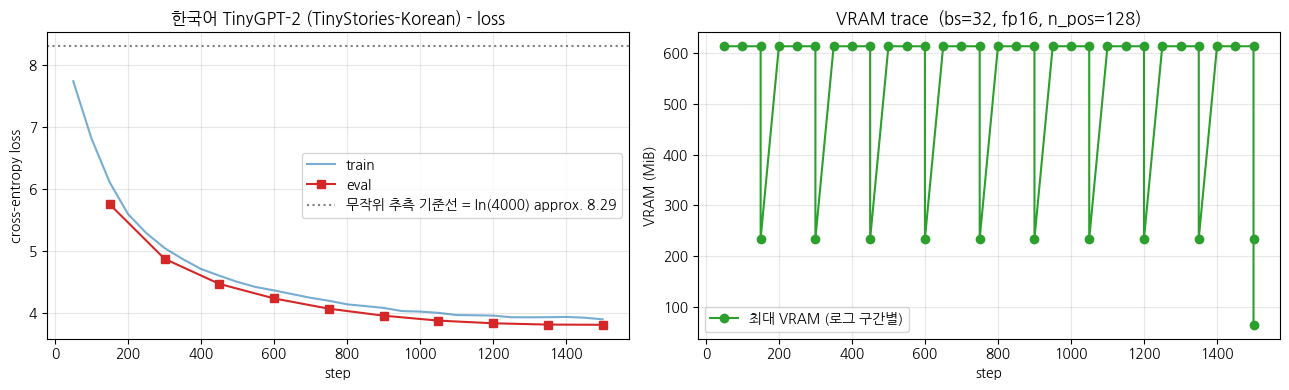
\includegraphics[width=0.88\linewidth]{assets/figures/ch26_loss_vram_trace.png}
\end{bookfigurelabel}

\textbf{그림 읽기} --- 그림~\ref{fig:ch26-loss-vram-trace}의 왼쪽 패널은 한국어 BBPE vocab 기준의 random baseline \inlinecode{ln(4000)} 근처에서 시작해 next-token loss가 빠르게 낮아지는 흐름을 보여줍니다. 오른쪽 패널은 \ref{ch:24}장과 같은 4-layer 구조가 vocab 4,000 설정에서 실측 4.22M params로 커져도 T4 VRAM 범위 안에서 안정적으로 학습되는지 확인하는 지표입니다.

\begin{bookfigurelabel}[H]{Scratch Causal LM의 영어/한국어 학습 손실 비교}{fig:ch26-ch24-loss-compare}
\includegraphics[width=0.72\linewidth]{assets/figures/ch26_ch24_loss_compare.png}
\end{bookfigurelabel}

\textbf{그림 읽기} --- 그림~\ref{fig:ch26-ch24-loss-compare}는 \ref{ch:24}장과 \ref{ch:26}장의 대칭 관계를 loss 관점에서 압축합니다. 한국어는 vocab 크기가 약 4,000으로 커져 random baseline이 조금 높지만, 학습 후 손실은 요약 \inlinecode{train\_loss=4.5487}, 마지막 logged loss 약 3.89 수준에 머뭅니다. 이 비교는 한국어 scratch 학습도 random baseline에서 빠르게 내려오지만, 영어 \ref{ch:24}장과 같은 2점대 수렴을 기대하면 안 된다는 점을 보여줍니다.



\textbf{관전 포인트} - 학습 첫 step loss 는 약 8.3 (random baseline \inlinecode{ln(4000)}) 부근에서 시작해 \emph{수백 step 안에 약 4-5} 로 빠르게 떨어집니다. 이번 실행본에서는 1500 step 요약 \inlinecode{train\_loss=4.5487}, 마지막 logged loss 약 3.89로 마무리됐습니다. 따라서 한국어 scratch 장의 정상 기준은 2점대가 아니라 \emph{4점대 초중반에서 계속 낮아지는 흐름} 입니다.



\section{\texorpdfstring{학습 \emph{후} generation + before/after 비교}{학습 후 generation + before/after 비교}}

같은 \inlinecode{PROMPTS\ /\ GEN\_KWARGS} 로 학습 후 모델에서 다시 생성하고, 앞에서 저장한 학습 전 결과와 나란히 비교합니다. \textbf{이 장의 합격 기준}: 학습 후 텍스트가 \emph{전} 보다 명확히 \emph{한국어 문장 (동화 풍)} 에 가까워졌는가 --- \ref{ch:24}장 (영어) 의 \emph{사전·사후 비교} 의 한국어판.



\Needspace{11\baselineskip}
\begin{lstlisting}
torch.manual_seed(SEED)
model.eval()
after_outputs = []
print("=" * 70)
print("TRAINED model - generation after Trainer.train()")
print("=" * 70)
for p in PROMPTS:
    text = generate_text(model, p, **GEN_KWARGS)
    after_outputs.append(text)
    print(f"\nprompt: {p}")
    print(text)
\end{lstlisting}

\Needspace{11\baselineskip}
\begin{lstlisting}
print("=" * 78)
print(
    "BEFORE (random init) vs AFTER (trained on "
    "TinyStories-Korean 30K)"
)
print("=" * 78)
for p, before, after in zip(PROMPTS, before_outputs, after_outputs):
    print(f"\nPROMPT  : {p}")
    print("-" * 78)
    print(f"BEFORE  : {before[len(p):].strip()[:280]}")
    print(f"AFTER   : {after[len(p):].strip()[:280]}")
\end{lstlisting}

\textbf{해석 가이드 - 사전학습이 만든 차이}

\begin{itemize}
\tightlist
\item
  \textbf{BEFORE (random init)}: \emph{한국어와 거리가 먼 음절·byte 조각 반복}. logits 가 random 초기값이라 sampling 이 통계적 빈도 토큰 사이에서만 흔들림.
\item
  \textbf{AFTER (한국어 TinyStories 30K \(\times\) 1500 steps)}: \emph{말이 되는 한국어 문장} - 짧지만 \emph{주어 + 서술어} 구조, \emph{동화 풍 어휘} (소녀, 친구, 엄마, 행복, 숲, 토끼, ...). 완벽하진 않아도 \emph{학습이 본체에 next-token 분포를 새긴 증거} 가 한 줄에서 명확.
\end{itemize}

\begin{quote}
\ref{ch:24}장 (영어) 의 \emph{사전·사후 generation 비교} 에서 random init 모델이 의미 없는 토큰을 뽑다가 학습 후 \emph{동화 풍 영어 문장} 을 만들어 낸 그 변화의 한국어판입니다. \emph{번역체 데이터} 라 영어판보다 다소 어색할 수 있지만, \emph{학습 전·후의 질적 도약} 자체는 동일하게 드러납니다.
\end{quote}



\section{변형 - sampling hyperparam / 더 큰 모델 / 더 많은 stories}

같은 한국어 prompt 에 \inlinecode{temperature\ /\ top\_k\ /\ top\_p} 만 바꿔 generation 스타일 변화 관찰. \emph{학습된 본체는 그대로} - 변하는 건 \emph{sampling 분포} 뿐.



\Needspace{11\baselineskip}
\begin{lstlisting}
prompt = "옛날 옛날에 작은 토끼가"
configs = [
    {"label": "T=0.3, top_k=20  (conservative)", "temperature": 0.3, "top_k": 20,  "top_p": None},
    {"label": "T=0.8, top_k=50  (balanced)",    "temperature": 0.8, "top_k": 50,  "top_p": None},
    {"label": "T=1.0, top_p=0.9 (nucleus)",     "temperature": 1.0, "top_k": 0,   "top_p": 0.9},
    {"label": "T=1.2, top_k=100 (diverse)",     "temperature": 1.2, "top_k": 100, "top_p": None},
]
for c in configs:
    torch.manual_seed(SEED)
    print("=" * 70)
    print(f"[{c['label']}]")
    print(generate_text(model, prompt, max_new_tokens=60, do_sample=True,
                        temperature=c["temperature"], top_k=c["top_k"], top_p=c["top_p"]))
    print()
\end{lstlisting}

\textbf{관전 포인트}

\begin{itemize}
\tightlist
\item
  \inlinecode{temperature} ↑ \(\to\) logits 분포 \emph{평탄화} \(\to\) 다양성 ↑, 일관성 ↓
\item
  \inlinecode{top\_k=20} \(\to\) 매 step 후보를 \emph{상위 20 개} 로만 한정 \(\to\) 안전하지만 반복적
\item
  \inlinecode{top\_p=0.9} (nucleus) \(\to\) 누적 확률 90\% 이내 후보 \(\to\) \emph{모델이 확신 있을 땐 좁게, 애매할 땐 넓게} 자동 조정
\item
  \inlinecode{T=1.2,\ top\_k=100} \(\to\) 가장 다양하지만 \emph{말이 안 되는 토큰} 도 종종 섞임
\end{itemize}

\textbf{더 큰 개선을 원하면} (T4 30분 룰 안):

\begin{booktable}{26장 변형 - sampling hyperparam / 더 큰 모델 / 더 많은 stories 표}{tab:ch26-10}
\begin{adjustbox}{max width=\textwidth}
\begin{tabular}{@{}llll@{}}
\toprule
변형 축 & 이 장 (기본) & 변형 예 & 예상 효과 \\
\midrule

\inlinecode{N\_TRAIN} (story 수) & 30,000 & 60,000 & 한국어 문장 자연스러움 ↑, 학습 시간 비례 증가 \\
\inlinecode{n\_embd} / \inlinecode{n\_layer} & 256 / 4 & 384 / 6 & 표현력 ↑ (약 8M params), T4 메모리 안에서 가능 \\
\inlinecode{max\_steps} & 1500 & 2500 & loss 추가 하락, 30분 룰 주의 \\
다른 한국어 코퍼스 & TinyStories-Korean & 한국어 위키 + 동화 혼합 & 도메인 폭 ↑, 단 어휘 난도 ↑ \\
\bottomrule
\end{tabular}
\end{adjustbox}
\end{booktable}



\section{(선택) Reference 비교 - KoGPT2 의 같은 prompt generation}

\emph{학습이 충분히 잘 된} 기준점으로 \inlinecode{skt/kogpt2-base-v2} (125M, 대규모 한국어 사전학습) 에 같은 한국어 prompt 를 넣어 \emph{우리 작은 GPT (4.22M, 한국어 TinyStories 30K)} 와 격차를 봅니다. \textbf{27장 이 KoGPT2 본격 장} 이므로 여기서는 \emph{간단히 한 번만} --- T4 시간을 아끼려면 이 셀은 건너뛰어도 됩니다.



\Needspace{11\baselineskip}
\begin{lstlisting}
RUN_KOGPT2_REF = True

if RUN_KOGPT2_REF:
    from transformers import AutoTokenizer, AutoModelForCausalLM

    print(
        "loading reference KoGPT2 (skt/kogpt2-base-v2, "
        "125M)..."
    )
    ref_tok = AutoTokenizer.from_pretrained("skt/kogpt2-base-v2")
\end{lstlisting}

\noindent\emph{앞 블록은 필요한 라이브러리와 기본 설정을 준비하는 단계입니다. 이어지는 블록에서는 앞에서 만든 중간 값을 다음 계산으로 넘기는 단계로 넘어갑니다.}

\Needspace{11\baselineskip}
\begin{lstlisting}[firstnumber=11]
    if ref_tok.pad_token is None:
        ref_tok.pad_token = ref_tok.eos_token
    ref_model = AutoModelForCausalLM.from_pretrained("skt/kogpt2-base-v2").to(device).eval()
    print(
        f"  #params : "
        f"{ref_model.num_parameters()/1e6:.1f} M"
    )

    torch.manual_seed(SEED)
    print("\n" + "=" * 70)
    print(
        "REFERENCE KoGPT2 (125M) - generation on same "
        "Korean prompts"
    )
    print("=" * 70)
\end{lstlisting}

\noindent\emph{앞 블록은 앞에서 만든 중간 값을 다음 계산으로 넘기는 단계입니다. 이어지는 블록에서는 텍스트를 모델 입력 텐서로 바꾸는 단계로 넘어갑니다.}

\Needspace{11\baselineskip}
\begin{lstlisting}[firstnumber=26]
    for p in PROMPTS:
        text = generate_text(
            ref_model,
            p,
            gen_tokenizer=ref_tok,
            **GEN_KWARGS,
        )
        print(f"\nprompt: {p}")
        print(text)

\end{lstlisting}

\noindent\emph{앞 블록은 텍스트를 모델 입력 텐서로 바꾸는 단계입니다. 이어지는 블록에서는 앞에서 만든 중간 값을 다음 계산으로 넘기는 단계로 넘어갑니다.}

\Needspace{10\baselineskip}
\begin{lstlisting}[firstnumber=36]
    del ref_model
    if torch.cuda.is_available():
        torch.cuda.empty_cache()
else:
    print(
        "Skipped KoGPT2 reference (RUN_KOGPT2_REF=False)."
        "Covered in depth in 27장."
    )
\end{lstlisting}

\textbf{해석 가이드 - 규모가 만든 격차}

\begin{itemize}
\tightlist
\item
  \textbf{OURS (4.22M, 한국어 TinyStories 30K)}: \emph{동화 풍 단순 한국어} - 어휘는 동화 도메인에 강하지만 \emph{복잡한 문장 구조 / 추상적 어휘} 는 약함.
\item
  \textbf{REF (KoGPT2 125M, 대규모 한국어 코퍼스)}: \emph{다양한 도메인 어휘 + 자연스러운 문장 흐름}. 학습 데이터의 규모·다양성이 generation 다양성으로 직결.
\end{itemize}

\begin{quote}
27장 이 이 격차를 \emph{데이터 축을 통제하고} 다룹니다 - KoGPT2 (125M) 의 사전학습 \emph{위에} 같은 한국어 TinyStories 로 \textbf{continual pretraining}. \emph{대규모 한국어 사전학습 모델을 작은 도메인 데이터로 적응} 시킬 때의 generation 품질이, 우리 from-scratch 작은 GPT 와 어떻게 다른지 직접 비교 (\ref{ch:24}장\(\to\)25 의 한국어 짝).
\end{quote}



\section{이 장에 등장한 라이브러리·함수 (\ref{ch:24}장과의 차이만)}

\begin{booktable}{26장 새로 등장한 라이브러리}{tab:ch26-11}
\begin{adjustbox}{max width=\textwidth}
\begin{tabular}{@{}lll@{}}
\toprule
이름 & 한 줄 설명 & \ref{ch:24}장과 차이 \\
\midrule

\inlinecode{load\_dataset("g0ster/TinyStories-Korean",\ streaming=True)} & 한국어 TinyStories 줄 단위 스트리밍 로드 & 영어 \(\to\) 한국어, story 복원 로직 추가 \\
\inlinecode{tokenizers.BPE\ +\ ByteLevel} (한국어 코퍼스) & byte-level BPE (BBPE) 직접 학습 & 학습 코퍼스 영어 \(\to\) 한국어, vocab 2,048 \(\to\) 약 4,000 \\
\inlinecode{AutoTokenizer.from\_pretrained("gpt2")} (비교용) & 영어 BPE 로 한국어 토큰화 비교 & 신규 (cross-language 실측) \\
\inlinecode{transformers.GPT2Config\ /\ GPT2LMHeadModel(config)} (동일) & 작은 GPT random init & (\ref{ch:24}장 동일, vocab 만 다름) \\
\inlinecode{DataCollatorForLanguageModeling(mlm=False)} (동일) & \inlinecode{labels\ =\ input\_ids.clone()} 자동 & (\ref{ch:24}장 동일) \\
\inlinecode{group\_texts} 패턴 (동일) & 가변 길이 \(\to\) 고정 length 블록 스트림 & (\ref{ch:24}장 동일) \\
\inlinecode{model.generate(do\_sample=True,\ ...)} (동일) & sampling generation & (\ref{ch:24}장 동일) \\
\inlinecode{AutoModelForCausalLM.from\_pretrained("skt/kogpt2-base-v2")} (선택) & KoGPT2 reference & gpt2 \(\to\) KoGPT2 \\
\bottomrule
\end{tabular}
\end{adjustbox}
\end{booktable}



\section{체크포인트 질문}

\begin{enumerate}
\def\labelenumi{\arabic{enumi}.}
\tightlist
\item
  영어 gpt2 BPE 로 한국어를 토큰화하면 토큰 수가 폭증합니다 (셀 비교 표). \emph{byte-level} 이라 UNK 는 없는데, 왜 그래도 \emph{직접 학습한 BBPE} 가 한국어 학습에 유리할까요? (의미 단위 보존 vs byte 조각 분해 관점)
\item
  random baseline 이 \ref{ch:24}장 (vocab 2,048) 의 \(\ln(2048) \approx 7.62\) 에서 \ref{ch:26}장 (vocab 약 4,000) 의 \(\ln(4000) \approx 8.29\) 로 바뀝니다. 이 차이가 \emph{학습 동역학} 에 의미 있는 영향을 주나요? \emph{학습 종료 loss 의 절대값} 을 영어 장과 비교할 때는요?
\item
  본 장의 collator 가 만드는 \inlinecode{labels} 는 \emph{거의 모든 자리} 가 학습 신호입니다. 28장 (한국어 SFT) 에서는 \texttt{labels{[}:prompt\_len{]}\ =\ -100} 한 줄로 \emph{prompt 부분만 제외} 합니다. \emph{왜 이 한 줄이 모델이 한국어 instruction 을 따라가게 만드는지} 설명해 보세요.
\item
  같은 본체 구조·loss·trainer 로 영어 (\ref{ch:24}장) 와 한국어 (\ref{ch:26}장) 를 학습했습니다. 학습 곡선·generation 품질이 두 언어에서 비슷하게 나온다면, \emph{언어 자체의 난도 차이} 와 \emph{데이터 규모·번역체 차이} 중 무엇이 generation 품질에 더 큰 영향을 줄까요?
\end{enumerate}



\section{FAQ}

\begin{faqBox}{Q1. (이론) 한국어 BBPE 는 영어 BPE 와 무엇이 다른가요? byte-level 이 한글을 어떻게 처리하나요?}

\textbf{알고리즘은 \emph{완전히 같습니다} --- 다른 건 \emph{학습 코퍼스} 뿐}. 둘 다 byte-level BPE (BBPE):

\begin{itemize}
\tightlist
\item
  \emph{가장 작은 단위가 byte (256개)} 라 한글·이모지·한자 \emph{어떤 유니코드도 UNK 없이} 표현.
\item
  한글 \inlinecode{가} 는 UTF-8 로 3 byte (\inlinecode{0xEA\ 0xB0\ 0x80}). BBPE 는 학습 중 \emph{자주 함께 등장하는 byte 쌍} 을 반복 병합해 \emph{글자·어절 단위} 토큰을 만듦.
\end{itemize}

차이는 \emph{어떤 코퍼스로 학습했는가}. 영어 코퍼스로 학습한 gpt2 BPE 는 \emph{영어 byte 패턴} 의 병합 규칙을 갖고 있어, 한국어를 넣으면 한글 byte 가 거의 \emph{원자 단위 그대로} 나와 토큰 수가 폭증합니다.

\Needspace{5\baselineskip}
\begin{lstlisting}
sent = "옛날 옛날에 작은 토끼가 살았어요."
len(gpt2_tok(sent, add_special_tokens=False)["input_ids"])
len(tokenizer(sent, add_special_tokens=False)["input_ids"])
\end{lstlisting}

한국어 코퍼스 위에 직접 학습하면 \emph{한국어 어절의 byte 패턴} 이 병합 규칙에 반영되어 \emph{훨씬 적은, 의미 있는 토큰} 으로 압축됩니다.

\end{faqBox}

\begin{faqBox}{Q2. (이론) 왜 한국어도 \emph{scratch} 부터 학습하나요? \ref{ch:24}장 (영어 scratch) 를 이미 했는데.}

\textbf{같은 시연 가치 + 한국어 특유의 필요성} 때문입니다.

\begin{enumerate}
\def\labelenumi{\arabic{enumi}.}
\tightlist
\item
  \emph{시연 가치} --- 사전학습이 본체에 \emph{next-token 분포} 를 새기는 과정을 \emph{한국어로} 직접 봅니다 (\ref{ch:20}장\(\to\)22 가 BERT 에서 한 것의 GPT 판).
\item
  \emph{한국어 특유의 필요성} --- 영어는 gpt2 BPE 를 그대로 가져다 continual pretraining (\ref{ch:25}장) 이 가능했지만, \emph{영어 BPE 는 한국어를 byte 조각으로 쪼개} 사실상 못 씁니다. 그래서 한국어는 \emph{토크나이저부터 새로} --- 자연스럽게 \emph{scratch} 가 됩니다.
\end{enumerate}

\Needspace{5\baselineskip}
\begin{lstlisting}
bbpe = Tokenizer(BPE(unk_token=None))
model = GPT2LMHeadModel(config)
\end{lstlisting}

\emph{토크나이저는 본체와 운명공동체} --- 토크나이저가 한국어를 못 다루면 본체 weight 도 유효한 신호를 받지 못합니다.

\end{faqBox}

\begin{faqBox}{Q3. (실무) 다음 장 (27장 KoGPT2 continual pretraining) 와의 관계는?}

27장 = \emph{대규모 한국어 사전학습 모델 KoGPT2 (\inlinecode{skt/kogpt2-base-v2}, 125M) 를 같은 한국어 TinyStories 로} \textbf{continual pretraining}. 본 장의 \emph{작은 from-scratch 모델} 과 \emph{완전 반대 출발점} --- \ref{ch:24}장\(\to\)25 (영어) 의 한국어 짝:

\begin{booktable}{26장 FAQ 표}{tab:ch26-12}
\begin{adjustbox}{max width=\textwidth}
\begin{tabular}{@{}lll@{}}
\toprule
축 & \ref{ch:26}장 (본 장) & 27장 (다음) \\
\midrule

모델 크기 & 4.22M params & \textbf{약 125M (약 30배)} \\
사전학습 & from scratch (random init) & \textbf{대규모 한국어 코퍼스 사전학습} \\
토크나이저 & 직접 학습 BBPE vocab 약 4,000 & \textbf{KoGPT2 BBPE (그대로)} \\
한국어 TinyStories 학습 & 사전학습 그 자체 (1500 steps) & \textbf{continual pretraining} (수백 steps) \\
Generation 품질 & 동화 풍 단순 한국어 & \textbf{자연스러운 동화 + 일반 도메인 폭} \\
\bottomrule
\end{tabular}
\end{adjustbox}
\end{booktable}

\textbf{핵심 메시지}: \emph{대규모 한국어 사전학습 본체} + \emph{작은 도메인 continual pretraining} 이 \emph{작은 from-scratch 모델} 보다 \emph{빠르게, 좋게} 도달합니다. \emph{왜 실무는 from-scratch 가 아니라 사전학습 모델을 가져와 계속 학습하는가} 의 한국어 답.

\end{faqBox}

\begin{faqBox}{Q4. (이론) 한국어 CausalLM 사전학습도 \inlinecode{labels\ =\ -100} 트릭을 쓰나요?}

\textbf{거의 안 씁니다 --- pad 자리만}. \ref{ch:24}장 (영어) 와 동일하게, 본 장 collator 출력은 \emph{거의 모든 자리} 가 학습 신호 (\inlinecode{labels\ =\ input\_ids.clone()}). \inlinecode{group\_texts} 로 chunk 길이가 모두 같으면 pad 도 없어 \inlinecode{-100} 이 0개일 수 있습니다.

같은 트릭이 \textbf{28장 (한국어 SFT)} 에서 \emph{결정적 한 줄} 로 부활합니다:

\Needspace{9\baselineskip}
\begin{lstlisting}
prompt = "### 질문: 한국의 수도는?\n### 답변: "
response = "서울입니다."

input_ids = tokenizer(prompt + response)["input_ids"]
labels = input_ids.copy()
prompt_len = len(tokenizer(prompt)["input_ids"])
labels[:prompt_len] = [-100] * prompt_len
\end{lstlisting}

이 한 줄로 모델은 \emph{prompt 를 외우지 않고 response 만 학습} \(\to\) \emph{주어진 instruction 에 response 를 생성} 하게 됩니다. 본 장의 collator 출력 (거의 모든 자리 = 학습 신호) 을 손에 익혀 두면 28장의 그 한 줄이 단번에 이해됩니다.

\end{faqBox}

\begin{faqBox}{Q5. (실무) 한국어 generation 품질이 영어 (\ref{ch:24}장) 보다 낮아 보이면 무엇을 의심하나요?}

세 가지 원인을 순서대로 점검합니다.

\begin{enumerate}
\def\labelenumi{\arabic{enumi}.}
\tightlist
\item
  \textbf{데이터 양·품질} --- \inlinecode{g0ster/TinyStories-Korean} 은 \emph{기계 번역본} 이라 원문 영어 TinyStories 보다 문장이 다소 어색하거나 일관성이 떨어질 수 있습니다. story 복원 (\texttt{\textless{}\textbar{}endoftext\textbar{}\textgreater{}} 기준) 이 제대로 됐는지, story 수가 충분한지 확인.
\end{enumerate}

\Needspace{5\baselineskip}
\begin{lstlisting}
print(raw_train[0]["text"][:300])
print(f"n_stories: {len(raw_train):,}")
\end{lstlisting}

\begin{enumerate}
\def\labelenumi{\arabic{enumi}.}
\setcounter{enumi}{1}
\item
  \textbf{토크나이저} --- vocab 약 4,000 이 너무 작으면 한 어절이 여러 byte 조각으로 쪼개져 학습이 어렵습니다. \inlinecode{VOCAB\_SIZE} 를 6,000-8,000 으로 키워 비교.
\item
  \textbf{학습량} --- \inlinecode{max\_steps} 또는 \inlinecode{N\_TRAIN} 을 키우면 한국어 문장 자연스러움이 올라갑니다 (T4 30분 룰 주의).
\end{enumerate}

\begin{quote}
\emph{번역체 데이터} 라 영어판보다 다소 어색한 건 \emph{정상} --- 본 장의 목표는 \emph{완벽한 한국어 생성} 이 아니라 \emph{학습 전·후의 질적 도약} 을 한국어로 확인하는 것. 자연스러운 한국어 generation 은 27장 (KoGPT2 continual pretraining) 의 영역.
\end{quote}

\end{faqBox}

\begin{faqBox}{Q6. (이론) \ref{ch:24}장 (영어) 와 \ref{ch:26}장 (한국어) 의 학습 곡선을 비교하려면?}

같은 hyperparam·같은 BLOCK\_SIZE·같은 step 수로 학습된 두 모델의 \emph{상대} 비교가 의미 있습니다.

\Needspace{8\baselineskip}
\begin{lstlisting}
metrics = {
    "language":          ["EN (24장)",  "KO (26장)"],
    "vocab_size":        [2048,          4000],
    "random_baseline":   [7.62,          8.29],
    "final_train_loss":  ["measure",     "measure"],
}
\end{lstlisting}

vocab 크기가 다르므로 \emph{random baseline (\inlinecode{ln\ V}) 이 다릅니다}. 절대 loss 를 직접 비교하기보다 \emph{random baseline 대비 얼마나 떨어졌는가} (상대 하락폭) 로 비교해야 공정합니다. 또 \emph{번역체 한국어} 는 원문 영어보다 \emph{반복·패턴} 이 적을 수 있어 같은 step 에서 loss 가 약간 높게 나올 수 있습니다 --- \emph{언어 난도} 보다 \emph{데이터 특성} 차이가 더 큽니다.

\end{faqBox}

\begin{faqBox}{Q7. (실무) 학습 첫 step loss 가 \(\ln(4000) \approx 8.29\) 가 아니라 \emph{5.0} 이라면? \emph{15.0} 이라면?}

\begin{itemize}
\tightlist
\item
  \textbf{5.0 (너무 낮음)}: vocab 크기 가정이 틀렸거나 (실제 vocab 이 더 작음), 토크나이저가 prompt 를 \emph{비정상적으로 적은 토큰} 으로 만들거나, 데이터가 \emph{극도로 반복적} 이어서 첫 배치가 쉬운 경우. \inlinecode{tokenizer.vocab\_size} 와 \inlinecode{math.log(tokenizer.vocab\_size)} 를 출력해 baseline 을 확인.
\end{itemize}

\Needspace{6\baselineskip}
\begin{lstlisting}
print(
    f"vocab: {tokenizer.vocab_size}, ln V = "
    f"{math.log(tokenizer.vocab_size):.2f}"
)
\end{lstlisting}

\begin{itemize}
\tightlist
\item
  \textbf{15.0 (너무 높음)}: \(\ln(4000) \approx 8.29\) 보다 훨씬 높다면 \emph{vocab 불일치} (모델 config 의 \inlinecode{vocab\_size} 와 토크나이저가 다름) 또는 \emph{입력 id 가 vocab 범위를 벗어남} 을 의심. \inlinecode{config.vocab\_size\ ==\ tokenizer.vocab\_size} 인지 점검하세요. random init 의 자연스러운 시작은 \emph{baseline 근처} 입니다.
\end{itemize}
\end{faqBox}



\begin{previewBox}{미리보기: 다음 장}

\textbf{27장. KoGPT2 Continual Pretraining 으로 한국어 TinyStories 에 적응 --- \emph{\ref{ch:25}장의 한국어판}}

\begin{itemize}
\tightlist
\item
  \inlinecode{AutoModelForCausalLM.from\_pretrained("skt/kogpt2-base-v2")} - 대규모 한국어 코퍼스로 사전학습된 125M params KoGPT2 로드
\item
  \textbf{같은 한국어 TinyStories} 데이터 (본 장와 동일) 로 \textbf{continual pretraining} (계속 사전학습 --- \emph{같은 CausalLM task, 새 데이터, head 그대로}. \emph{task adaptation 의미의 fine-tune 이 아니라 단계 2})
\item
  \textbf{핵심 비교}: 본 장 (4.22M, from scratch) vs 27장 (125M, continual pretraining) 의 한국어 generation 품질·학습 곡선 격차
\item
  \emph{trainer 자체는 \ref{ch:26}장과 동일} (\inlinecode{transformers.Trainer} + \inlinecode{DataCollatorForLanguageModeling(mlm=False)}) - \emph{변하는 건 모델 로드 한 줄 + lr (scratch 5e-4 \(\to\) continual pretraining 2e-5)}
\item
  \ref{ch:24}장\(\to\)\ref{ch:25}장 (영어) 의 한국어 짝 - \emph{왜 실무가 from-scratch 가 아니라 대규모 사전학습 모델 위에 계속 학습하는가} 의 한국어 정량 답변
\end{itemize}

\begin{quote}
\textbf{변하는 축}: \emph{모델 크기 + 사전학습 여부} (4.22M / scratch \(\to\) 125M / pretrained). 데이터·토크나이저 규약·loss·trainer 는 같음. Phase 4 의 \emph{학습 단계 2 (continual pretraining)} 가 한국어에서 자리 잡는 장. \emph{진짜 행동 정렬 (SFT)} 은 28장에서 본격 등장합니다.
\end{quote}
\end{previewBox}
